\section{Introduction}
\label{sec:intro}

Cloud service systems consume a growing fraction of global electricity, and carbon-aware scheduling is increasingly central to green-ICT research~\cite{patel2024modeling,gill2024modern}. FaaS is the dominant delivery model on the cloud--edge continuum; each invocation is individually schedulable~\cite{calavaro2025beyond,russo2024qosaware}. The natural lever for carbon-aware orchestrators is \emph{deferral}: a deadline-elastic invocation is held back and executed later, when the grid is cleaner~\cite{asadov2025carbonaware,patel2024agile,gsteiger2024caribou}.

Two assumptions in that body of work are jointly wrong. First, existing schedulers use the \emph{average} carbon intensity, but when a workload is deferred, the incremental electricity is marginal---it is served by the generator that ramps to meet the load. Using the average signal systematically misranks deferral targets and can increase emissions~\cite{sukprasert2024implications,maji2024green}. Second, carbon-aware schemes use either greedy scheduling or long-horizon forecasts, but neither matches how renewable surpluses arrive: as short, weather-driven windows that last minutes to hours~\cite{chen2024towards}. A greedy scheduler misses the cleaner window that opens an hour later; a long-forecast scheduler knows a clean window exists on average but not within the job's deadline. We argue that the scheduler should use a real-time \emph{marginal} signal, forecast an imminent surplus window, and charge embodied carbon when a warm instance is reused.

\begin{figure}[tb]
\centering
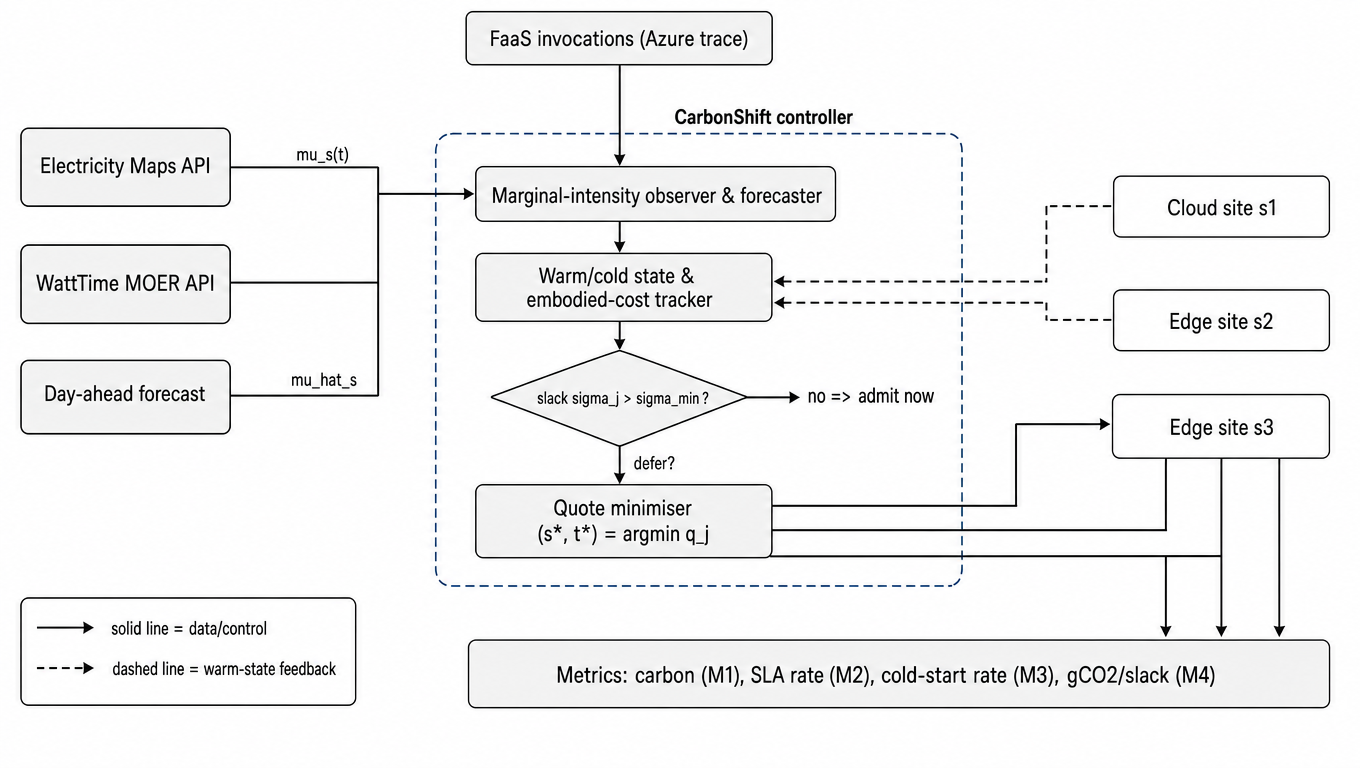
\includegraphics[width=\columnwidth]{figures/framework_render.png}
\caption{The \textsc{CarbonShift} framework. External marginal-intensity
signals (left) and FaaS invocations (top) enter the controller, which
observes current and forecast marginal intensity, tracks the warm/cold
and embodied-cost state of each eligible site, decides whether the
slack admits deferral, and commits the placement minimising the carbon
quote of Eq.~\eqref{eq:quote} to a cloud or edge site (right). Dashed
arrows return the warm-state feedback that drives embodied amortisation.}
\label{fig:framework}
\end{figure}

Figure~\ref{fig:framework} previews the \textsc{CarbonShift} framework. The controller consumes a real-time marginal MOER signal and a short-horizon surplus forecast, tracks the warm/cold state of each eligible site, and commits the placement that minimises the carbon quote of Eq.~\eqref{eq:quote}.

This paper makes three contributions. First, we formalise marginal-carbon-aware serverless deferral as an online problem with deadline-elastic FaaS invocations and per-site embodied-carbon costs. Second, we give a competitive algorithm with three guarantees: (i)~a competitive bound that collapses to a small constant on real grid sequences, (ii)~a slack-safety threshold, and (iii)~a non-gameability theorem. Third, we evaluate the controller on the Azure Functions~2019 trace paired with real WattTime CAISO\_NORTH MOER data (72~h, 864 points). Across three seeds, \textsc{CarbonShift} reduces M1 by 4--6\% versus Greedy; the marginal signal is worth 0.5--0.6~pp of M1; and the inflated-deadline charged cost is 21\% higher than the honest report.
